\documentclass[margin=0cm]{standalone}

\PassOptionsToPackage{dvipsnames}{xcolor}
\usepackage{amsmath}
\usepackage{amsfonts}
\usepackage{tikz}
\usetikzlibrary{arrows.meta}
\usetikzlibrary{calc}
\usetikzlibrary{decorations.markings}
\tikzset{
    every node/.style={align=center},
}

\begin{document}
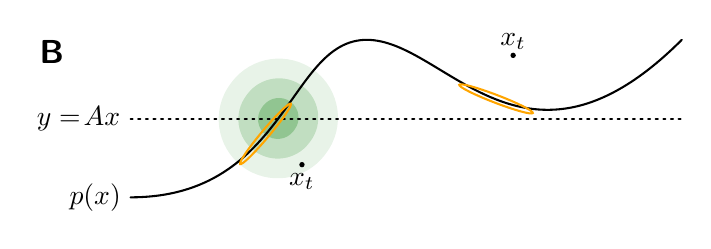
\begin{tikzpicture}
    \node[below, inner sep=0] at (-1.0, 2.0) {\large\textbf{\textsf{B}}};

    \path[
        save path=\M,
        postaction={decorate,
            decoration={markings,
                mark=between positions 0 and 1 step 0.001 with {
                    \coordinate (x\pgfkeysvalueof{/pgf/decoration/mark info/sequence number});
                    \coordinate (n\pgfkeysvalueof{/pgf/decoration/mark info/sequence number}) at (0.0, 0.6);
                }
            }
        }
    ] (0.0, 0.0) node[left] {$p(x)$} .. controls +(2.0, 0.0)
        and +(-1.0, 0.0) .. (3.0, 2.0) .. controls +(1.0, 0.0)
        and +(-2.0, -2.0) .. (7.0, 2.0);

    \path[save path=\segment] (x264) -- (x267);
    \draw[use path=\segment, ForestGreen, opacity=0.1, line cap=round, line width=1.5cm];
    \draw[use path=\segment, ForestGreen, opacity=0.2, line cap=round, line width=1.0cm];
    \draw[use path=\segment, ForestGreen, opacity=0.3, line cap=round, line width=0.5cm];

    \draw[use path=\M, line cap=round, line width=0.75pt];
    \draw[dotted, line cap=round, line width=0.75pt] (0.0, 1.0) node[left] {$y=\!Ax$} -- (7.0, 1.0);

    % Left mode
    \coordinate (xt) at ($(x235)!-1!(n235)$);
    \coordinate (x_xt) at ($(x235)!0.01!(n235)$);

    \filldraw (xt) circle (0.75pt) node[below, inner sep=3pt] {$x_t$};
    \draw[Orange, rotate=50, line width=0.75pt] (x_xt) ellipse (0.5 and 0.05);

    % Right mode
    \coordinate (xt) at (n670);
    \coordinate (x_xt) at ($(x670)!0.01!(n670)$);

    \filldraw (xt) circle (0.75pt) node[above, inner sep=2pt] {$x_t$};
    \draw[Orange, rotate=-21, line cap=round, line width=0.75pt] (x_xt) ellipse (0.5 and 0.05);
\end{tikzpicture}
\end{document}